\documentclass[french, 12pt]{article}

\usepackage[utf8]{inputenc}    % Encodage
\usepackage[T1]{fontenc}       % Encodage des polices
\usepackage{lipsum}            % Générateur de texte pour les exemples
\usepackage{graphicx}          % Pour inclure des images
\usepackage{amsmath}           % Pour les formules mathématiques
\usepackage{amsfonts}          % Pour les polices mathématiques
\usepackage{amssymb}           % Pour les symboles mathématiques
\usepackage{hyperref}          % Pour les liens
\usepackage{fancyhdr}          % Pour les en-têtes et pieds de page
\usepackage{xcolor}

% Configuration de l'en-tête et du pied de page
\pagestyle{fancy}
\fancyhf{}
\fancyhead[L]{Sokoban}
\fancyhead[R]{Sacha David et Nathael Carlier}     
\fancyfoot[C]{\thepage}        

% Titre et auteur
\title{Projet Sokoban}
\author{Sacha David et Nathael Carlier\\
        Prép'Isima 2}
\date{\today}




% détaillant la modélisation du jeu (choix retenus pour la modélisation du plateau, 
%des éléments ainsi que les strutures de données. À des fins d’évaluations, il sera précisé comment lancer le programme.)
\begin{document}

\maketitle

\tableofcontents

\section{Introduction}

    Le but de ce projet est de recréer le jeu \href{https://fr.wikipedia.org/wiki/Sokoban}{Sokoban} en utilisant le language de programmation C. 

    C'est un jeu ou le joueur doit ranger des caisses sur des cases cibles. Il peut se déplacer dans les quatre directions, et seulement pousser (pas tirer) une seule caisse à la fois. Une fois toutes les caisses rangées, le niveau est réussi et le joueur passe au niveau suivant, plus difficile en général. L'idéal est de réussir avec le moins de déplacement possibles. En principe le personnage de ce jeu est un gardien d'entrepôt rangeant les caisses d'un entrepôt à leur bon endroit. Sokoban ressemble en général à l'illustration ci-dessus (mais comme vous allez le voir nous avons pris quelque liberter de design).

    \begin{figure}[h]
        \centering
        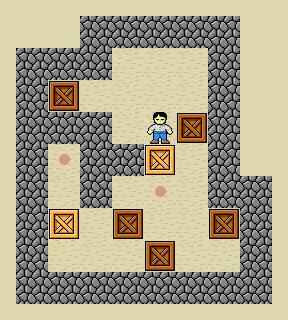
\includegraphics[width=0.4\textwidth]{illustration/base_sokoban.png}
        \caption{Exemple typique d'un jeu sokoban}
    \end{figure}

\section{Nécessaire pour le lancement du jeu}

Pour cette section on vous renvoie sur la \href{../doc/redirect.html}{page d'accueil} de notre documentation expliquant la démarche a suivre pour compiler et éxécuter le jeu.

\section{Choix de  modélisation} % Ou D.A. jsp pas quoi mettre 

    \subsection{Explication}
        Nous avons remarqué que les graphismes du jeu de base était trop basiques et pas forcément jolies. C'est pour cela que nous avons décider de complétement changer la direction artistique de notre jeu pour donner un cotê plus mignon au jeux.

    \subsection{Changements}
        Le personnage ne sera plus un gardien d'entrepôt mais un \href{https://fr.wikipedia.org/wiki/Hydrochoerus_hydrochaeris}{capybara} et lieu dans lequel le jeu ce déroule sera une étendu d'eau en bas d'une casquade. Notre personnage ne déplacera pas de caisse sur leur rangement mais il déplacera des oranges sur des nénuphars. 
        Deplus les murs en pierre n'existeront pas, ce sera des rochers dépassant de l'eau, le tout avec un rendu en isométrique.

        % Mettre image montrant la différence entre les deux


\section{Structuration du jeu}

    \subsection{Grille de jeu}
        La grille de jeu est la carte où le personnage (joueur) peut ce déplacer et interragir avec les éléments présent. Chaque niveau a une carte différente.

        Nous avons décider de stocker les cartes des niveaux dans des fichiers texte (.txt) différent, ces fichiers sont tous nommée 'map' puis leur numéro de niveau. Par exemple 'map1.txt' est la carte du premier niveau. \\
        Un fichier est organisé de manière à former un tableau de lettre et d'espace où chaque charactère représente un élément. La position des charactère dans le fichier et dans le jeu seront les mêmes (au début).
        \begin{itemize}
            \item 'W': Wall, représenté par rocher.
            \item 'C': Caisse, représenté par une orange (que le joueur devra pousser).
            \item 'I': Interest point, représenté par un nénuphar (qui accueillera une orange).
            \item 'P': Player, représenté par un Capybara.
            \item 'F': Rocks with Frog, représente un type de rochers particulié.
            \item ' ': Void, ce sont les cases où il y a rien.\\
        \end{itemize}

        Pour l'instant la grille de jeu présent dans le fichier est inutilisable par un programme. C'est pour ça que l'on va stocker le contenu de celui-ci dans un tableau.

        Mais tout d'abord laissé moi vous présenter la structure qui va accueillir notre grille de jeu et pas que. Nous avons nommé cette structure \textcolor{blue}{\textbf{Map}}. Elle contient plusieurs attribut expliqués dans la {docummentation}, ici nous allons nous concentré sur les attribut utile à l'exécution du jeu et non à l'affichage des textures. \\

        \textcolor{blue}{\textbf{Map}} stocke 2 tableaux de 2 dimensions représentant les grilles de jeu. Il y a un tableau stockant tout les éléments du jeu et un autre qui stocke aussi la grille de jeu mais il stocke seulemnt les cases de vides et les points d'intérets. Le premier tableau représente la carte a tout moment de jeu, ce tableau change à chaque action du joueur. Tandis que le deuxième tableau ne change pas durant toutes la partie, en effet il stocke la grille de jeu à l'état initial. Il va servir entre autre de repaire pour vérifier si les points d'intérets sont complété.\\
        Pour pouvoir correctement lire ces tableaux il faut connaitre leur nombre de ligne et colonne, c'est pour ça que \textcolor{blue}{\textbf{Map}} stocke ces données. Cette structure stocke aussi le numéro de la carte, cela permet de changer de carte plus facilement.

    \subsection{Joueur}
        La structure \textcolor{blue}{\textbf{Map}} vu précédement suffit a stocker toutes les informations utiles pour le fonctionnnement du jeu. Malgré cela nous avons décider de créer une structure pour représenter le personnage \textcolor{blue}{\textbf{Player}}.

        Cette structure stocke principalement des informations utile à l'affichage du personnage. Malgré cela elle stocke la position du joueur en i et j (y et x pour un plan mathématique). Ce stockage facilite les mouvements du joueur puisque l'on n'a pas besoin de chercher la position du joueur à chacun de ses déplacements.

    \subsection{Interaction}
        Nous avons définis les éléments du jeu et leur structuration, il nous faut dès à présent définir les interactions entre ces éléments.
        \\
        Le joueur et les caisses sont les seuls éléments a ce déplacer. En effet le principe du jeu \textbf{Sakoban} est de déplacer des boites jusqu'à un endroit clé, donc ce sont que les caisses et le joueur qui ce déplace. Pour ce faire le personnage peut ce déplacer et déplacer des caisses. Ces déplacements ont quelques contraintes:

        \begin{itemize}
            \item[$-$] Le joueur ne peut ni traverser de mur ni traverser de caisse (orange).
            \item[$-$] Une caisse a les mêmes conntraintes que le joueur.
            \item[$-$] Le joueur et les caisses ne peuvent pas sortir de la carte.
            \item[$-$] Une caisse est déplacable uniquement par le joueur.
            \item[$-$] Le joueur pousse une caisse dans la direction de son déplacement.
        \end{itemize}


\section{Affichage du jeu}
% Comment on affiche le tout 

% Récap arboresence projet
\section{Conclusion}



\end{document}
